\chapter{TINJAUAN PUSTAKA}
\section{Hasil Penelitian Terdahulu}
\begin{table}[H]
  \centering
  \begin{tabular}{|c|m{4cm}|c|m{8cm}|}
    \hline
    \textbf{No} & \textbf{Peneliti}                                          & \textbf{Tahun}                                   & \textbf{Hasil Penelitian}                                                                                             \\ \hline
    1           & \citeauthorfullname{mufid2014eigenvalues}                  & \citeyear{mufid2014eigenvalues}                  & Menyelesaikan permasalahan nilai eigen dan vektor eigen dari Latin square pada aljabar max-plus.                      \\ \hline
    2           & \citeauthorfullname{linde2014matricescommutinggivennormal} & \citeyear{linde2014matricescommutinggivennormal} & Menyatakan syarat perlu dan cukup bagi dua matriks tropikal agar komutatif berdasarkan nilai diagonal utama.          \\ \hline
    3           & \citeauthorfullname{trivialeigenvectorsym14061101}         & \citeyear{trivialeigenvectorsym14061101}         & Mengkaji sifat-sifat vektor eigen trivial pada aljabar max-plus.                                                      \\ \hline
    4           & \citeauthorfullname{zufar2023konstruksigrup}               & \citeyear{zufar2023konstruksigrup}               & Mengkonstruksi grup Latin square pada aljabar max-plus dengan operasi perkalian matriks tropikal.                     \\ \hline
    5           & \citeauthorfullname{alhussaini2024securityinitialtropical} & 2024                                             & Memperkenalkan protokol kriptografi berbasis aljabar tropikal yang terinspirasi dari pertukaran kunci Diffie-Hellman. \\ \hline
  \end{tabular}
\end{table}
\section{Aljabar Max-Plus}
Aljabar max-plus salah satu cabang dari aljabar tropikal yang menggunakan operasi maksimum dan penjumlahan sebagai operasi dasar.
\begin{definisi}[\cite{subiono2015minmaxplus}]
  Aljabar max-plus adalah himpunan $\mathbb{R}_{\max} = \mathbb{R} \cup \{\varepsilon\}$ dengan $\varepsilon=-\infty$ yang dilengkapi dengan dua operasi biner yaitu:
  \begin{align*}
    a \oplus b  & = \max\{a, b\}, \quad \forall a, b \in \mathbb{R}_{\max} \\
    a \otimes b & = a + b, \quad \forall a, b \in \mathbb{R}_{\max}
  \end{align*}
  yang elemen identitasnya adalah $\varepsilon$ untuk operasi $\oplus$ dan $0$ untuk operasi $\otimes$.
\end{definisi}

Selanjutnya $(\mathbb{R}_{\max}, \oplus, \otimes)$ disebut sebagai semiring max-plus, yaitu suatu struktur aljabar yang memenuhi sifat seperti ring biasa, kecuali tidak memiliki elemen invers untuk operasi $\oplus$.

\subsection{Matriks Aljabar Max-Plus}
Pada aljabar max-plus, matriks juga dapat didefinisikan dengan menggunakan operasi penjumlahan dan perkalian pada aljabar max-plus. Sebuah matriks bisa dianggap sebagai representasi dari suatu sistem diskrit atau graf berarah berbobot, sehingga dapat digunakan untuk memodelkan berbagai permasalahan matematika \parencite{subiono2015minmaxplus}.
\begin{definisi}[\cite{Baccelli1994maxplus}]
  Misalkan $A = (a_{ij})$ adalah matriks berukuran $m \times n$ dan $B = (b_{ij})$ adalah matriks berukuran $n \times p$ dengan elemen-elemen dari $\mathbb{R}_{\max}$. Operasi penjumlahan dan perkalian matriks pada aljabar max-plus didefinisikan sebagai berikut:
  \begin{align*}
    (A \oplus B)_{ij}  & = a_{ij} \oplus b_{ij} = \max\{a_{ij}, b_{ij}\}                                          \\
    (A \otimes B)_{ij} & = \bigoplus_{k=1}^{n} a_{ik} \otimes b_{kj} = \max_{1 \leq k \leq n} \{a_{ik} + b_{kj}\}
  \end{align*}
\end{definisi}

\begin{contoh}
  Misalkan diberikan matriks $A$ dan $B$ sebagai berikut:
  \[
    A = \begin{pmatrix}
      2 & 3 \\
      5 & 1
    \end{pmatrix}, \quad
    B = \begin{pmatrix}
      4 & 0 \\
      2 & 6
    \end{pmatrix}
  \]
  Maka, penjumlahan dan perkalian matriks $A$ dan $B$ pada aljabar max-plus adalah:
  \begin{align*}
    A \oplus B  & = \begin{pmatrix}
                      \max\{2, 4\} & \max\{3, 0\} \\
                      \max\{5, 2\} & \max\{1, 6\}
                    \end{pmatrix} = \begin{pmatrix}
                                      4 & 3 \\
                                      5 & 6
                                    \end{pmatrix}              \\
    A \otimes B & = \begin{pmatrix}
                      \max\{2 + 4, 3 + 2\} & \max\{2 + 0, 3 + 6\} \\
                      \max\{5 + 4, 1 + 2\} & \max\{5 + 0, 1 + 6\}
                    \end{pmatrix} = \begin{pmatrix}
                                      6 & 9 \\
                                      9 & 7
                                    \end{pmatrix}
  \end{align*}
  Dari hasil di atas, dapat didefinisikan matriks identitas terhadap operasi $\otimes$ yaitu
  \[
    I_n =
    \begin{pmatrix}
      0           & \varepsilon & \cdots & \varepsilon \\
      \varepsilon & 0           & \cdots & \varepsilon \\
      \vdots      & \vdots      & \ddots & \vdots      \\
      \varepsilon & \varepsilon & \cdots & 0
    \end{pmatrix}
  \]
  dengan $n$ adalah ordo matriks identitas tersebut. Oleh karena itu, setiap matriks $A\in \mathbb{R}_{\max}^{n \times n}$ akan memenuhi $A \otimes I_n = I_n \otimes A = A$.
\end{contoh}

\subsection{Polinomial dalam Aljabar Max-Plus}
Polinomial adalah suatu ekspresi matematika yang terdiri dari variabel dan koefisien, yang dioperasikan dengan penjumlahan, pengurangan, dan perkalian. Dalam aljabar max-plus, polinomial juga dapat didefinisikan dengan menggunakan operasi maksimum dan penjumlahan pada aljabar max-plus \parencite{burden2010numerical}.
\begin{definisi}[\cite{muanalifah2020modifyingtropical}]
  Polinomial max-plus atau tropikal adalah sebuah fungsi $x\mapsto p(x)$ yang didefinisikan sebagai
  \[
    p(x) = \bigoplus_{k=0}^{n} a_{k} \otimes x^{\otimes k} = \max_{0 \leq k \leq n} \{a_{k} + kx\},
  \]
  dengan $a_k \in \mathbb{R}_{\max}$ untuk setiap $k = 0, 1, \ldots, n$.
\end{definisi}
\subsection{Matriks Linde-de la Puente}
Berdasarkan hasil penelitian \textcite{linde2014matricescommutinggivennormal}, diperoleh bahwa kekomutatifan antara dua matriks tropikal sangat bergantung pada diagonal utama matriks tersebut. Dalam perkembangan selanjutnya, \textcite{alhussaini2024securityinitialtropical} memperkenalkan juga sebuah protokol kriptografi yang terinspirasi dari pertukaran kunci Diffie-Hellman, yang basisnya adalah grup siklik $(\Z_p^*\ ,\ \times)$ untuk suatu bilangan prima $p$.
\begin{definisi}[\cite{alhussaini2024implementationstickel}]
  Untuk setiap bilangan real $r \leq 0$ dan bilangan real $k \geq 0$, kita definisikan
  $
    [2r, r]_{n}^{k}
  $
  sebagai himpunan matriks $A_{n\times n}$ sedemikian sehingga $a_{ii} = k$ untuk semua $i$ dan $a_{ij} \in [2r, r]$ untuk $i \neq j$.
\end{definisi}
dari definisi di atas diperoleh sebuah teorema penting mengenai kekomutatifan matriks tropikal.
\begin{teorema}[\cite{alhussaini2024securityinitialtropical}]
  Misalkan $A \in [2r, r]_{n}^{k_{1}}, \, B \in [2s, s]_{n}^{k_{2}}$ untuk setiap $r, s \leq 0$ dan $a_{ii} = k_{1} \geq 0, \, b_{ii} = k_{2} \geq 0$. Maka
  \[
    A \otimes B = B \otimes A = k_{2} \otimes A \oplus k_{1} \otimes B.
  \]
  \begin{contoh}
    Misalkan diberikan matriks $A\in [-4, -2]_{2}^{3}$ dan $B\in [-3, -1]_{2}^{2}$ sebagai berikut:
    \[
      A =
      \begin{pmatrix}
        3  & -2 & -4 \\
        -3 & 3  & -2 \\
        -2 & -4 & 3
      \end{pmatrix},
      \quad
      B =
      \begin{pmatrix}
        2  & -1 & -3 \\
        -3 & 2  & -1 \\
        -1 & -3 & 2
      \end{pmatrix}.
    \]
    Dengan menggunakan operasi pada aljabar max-plus, diperoleh
    \begin{align*}
      A \otimes B & =
      \begin{pmatrix}
        5 & 2 & 0 \\
        0 & 5 & 2 \\
        2 & 0 & 5
      \end{pmatrix},  \quad
      B \otimes A  =
      \begin{pmatrix}
        5 & 2 & 0 \\
        0 & 5 & 2 \\
        2 & 0 & 5
      \end{pmatrix}.
    \end{align*}
    Sehingga, $A$ dan $B$ komutatif terhadap operasi $\otimes$.
  \end{contoh}
\end{teorema}

\section{Grup}
Dalam aljabar abstrak, grup adalah himpunan yang dilengkapi dengan suatu operasi biner yang memenuhi empat aksioma dasar \parencite{subiono2022aljabar}. Misalkan $G$ adalah himpunan dan $*$ adalah operasi biner pada $G$, maka $(G, *)$ disebut grup jika memenuhi sifat-sifat berikut:
\begin{itemize}
  \item \textbf{Tertutup}: Untuk setiap elemen $a, b$ dalam himpunan $G$, hasil operasi $a * b$ juga merupakan elemen dari $G$.
  \item \textbf{Asosiatif}: Untuk setiap elemen $a, b, c$ dalam himpunan $G$, berlaku $(a * b) * c = a * (b * c)$.
  \item \textbf{Identitas}: Terdapat elemen identitas $e$ dalam himpunan $G$ sehingga untuk setiap elemen $a$ dalam $G$, berlaku $e * a = a * e = a$.
  \item \textbf{Invers}: Untuk setiap elemen $a$ dalam himpunan $G$, terdapat elemen invers $a^{-1}$ dalam $G$ sehingga $a * a^{-1} = a^{-1} * a = e$.
\end{itemize}
\begin{contoh}[\cite{subiono2022aljabar}]
  Grup yang akan dibahas dalam penelitian ini adalah grup permutasi $S_n$, yaitu himpunan semua permutasi dari himpunan $\{1, 2, \ldots, n\}$ dengan operasi komposisi fungsi. Grup dari himpunan $S_n$ terhadap operasi perkalian permutasi (komposisi fungsi) dinamakan
  grup simetri berderajad $n$.
\end{contoh}

\subsection{Homomorfisma dan Isomorfirsma Grup}
Homomorfisma grup adalah suatu pemetaan antara dua grup yang mempertahankan struktur grup tersebut. Misalkan $(G, *)$ dan $(H, \cdot)$ adalah dua grup, maka suatu fungsi $f: G \to H$ disebut homomorfisma grup jika untuk setiap elemen $a, b$ dalam $G$, berlaku
\[
  f(a * b) = f(a) \cdot f(b).
\]
Jika homomorfisma $f$ bersifat bijektif (satu-satu dan pada), maka $f$ disebut isomorfisma grup. Dua grup misalkan $G$ dan $H$ dikatakan isomorfik jika terdapat isomorfisma antara keduanya dan dinotasikan sebagai $G\cong H$. Isomorfik menunjukkan bahwa kedua grup tersebut memiliki struktur yang sama meskipun elemen-elemennya berbeda \parencite{subiono2022aljabar}.

\section{Permutasi}
Dalam aljabar, permutasi ialah suatu fungsi bijektif dari himpunan ke dirinya sendiri. Sebuah permutasi dari himpunan $X = \{1, 2, \ldots, n\}$ biasanya disimbolkan dengan $\sigma: X \to X$, dengan $\sigma$ bersifat satu-satu dan pada. Himpunan semua permutasi dari $X$ membentuk suatu grup terhadap operasi komposisi fungsi, yang disebut grup simetris pada $n$ elemen yang disimbolkan dengan $S_n$ \parencite{subiono2022aljabar}.
\begin{contoh}
  Misalkan diberikan himpunan $X = \{1, 2, 3\}$. Salah satu permutasi dari himpunan $X$ adalah fungsi $\sigma$ yang didefinisikan sebagai berikut:
  \[
    \sigma(1) = 2, \quad \sigma(2) = 3, \quad \sigma(3) = 1
  \]
  atau dapat dituliskan dalam bentuk sebuah matriks berikut
  \[
    \sigma = \begin{pmatrix}
      1 & 2 & 3 \\
      2 & 3 & 1
    \end{pmatrix}
  \]
\end{contoh}
\subsection{Sikel}
Misalkan $\tau$ adalah permutasi pada himpunan $X = \{1,2,\ldots,n\}$.
Untuk suatu elemen $i_1 \in X$, perhatikan barisan
$
  (i_1,\ \tau(i_1),\ \tau^2(i_1),\ \ldots).
$
Karena himpunan $X$ berhingga, terdapat bilangan $k \ge 1$ sehingga
$
  \tau^{k}(i_1) = i_1.
$
Himpunan
\[
  \mathcal{O}_{\tau}(i_1)
  =
  \{\, i_1,\ \tau(i_1),\ \tau^{2}(i_1),\ \ldots,\ \tau^{k-1}(i_1)\,\}
\]
disebut \emph{orbit} dari $\tau$ yang melalui $i_1$.
Orbit menggambarkan lintasan elemen $i_1$ di bawah penerapan berulang dari permutasi $\tau$ \parencite{subiono2022aljabar}.

\begin{definisi}
  Jika orbit $\mathcal{O}_{\tau}(i_1)$ memuat lebih dari satu elemen, maka orbit tersebut disebut
  \emph{sikel} dari permutasi $\tau$. Dalam notasi siklus, sikel tersebut dituliskan sebagai
  \[
    (i_1\ i_2\ \ldots\ i_k),
  \]
  yang menyatakan bahwa
  \[
    \tau(i_j) = i_{j+1} \quad \text{untuk } 1 \le j < k,
    \qquad
    \tau(i_k) = i_1.
  \]
\end{definisi}

\begin{teorema}[\cite{subiono2022aljabar}]
  Setiap permutasi $\tau\in S_n$ dapat dituliskan sebagai hasil komposisi dari sikel-sikel yang saling asing.
\end{teorema}

Dengan menggunakan notasi sikel, permutasi akan lebih ringkas untuk dituliskan dan dipahami.

\begin{contoh}
  Misalkan diberikan permutasi $\tau\in S_9$ yang didefinisikan
  \begin{align}
    \tau=\begin{pmatrix}
           1 & 2 & 3 & 4 & 5 & 6 & 7 & 8 & 9 \\
           3 & 1 & 2 & 5 & 4 & 6 & 8 & 7 & 9
         \end{pmatrix}.
  \end{align}
  Dengan menggunakan notasi sikel, permutasi $\tau$ dapat dituliskan sebagai
  \[
    \tau = (1\ 3\ 2)(4\ 5)(6)(7\ 8)(9).
  \]
  \begin{figure}[H]
    \centering
    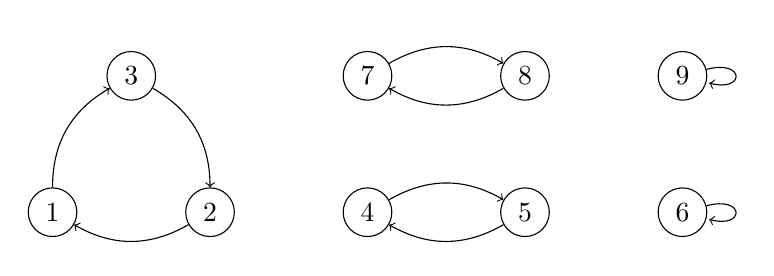
\begin{tikzpicture}[scale=1]
      \node[circle, draw] (1) at (0, 0) {1};
      \node[circle, draw] (2) at (2, 0) {2};
      \node[circle, draw] (3) at (1, 1.732) {3};
      \node[circle, draw] (4) at (4, 0) {4};
      \node[circle, draw] (5) at (6, 0) {5};
      \node[circle, draw] (6) at (8, 0) {6};
      \node[circle, draw] (7) at (4, 1.732) {7};
      \node[circle, draw] (8) at (6, 1.732) {8};
      \node[circle, draw] (9) at (8, 1.732) {9};

      \draw[->] (1) to[bend left] node[above] {} (3);
      \draw[->] (3) to[bend left] node[above] {} (2);
      \draw[->] (2) to[bend left] node[above] {} (1);

      \draw[->] (4) to[bend left] node[above] {} (5);
      \draw[->] (5) to[bend left] node[above] {} (4);

      \path (6) edge[->, loop right] ();

      \draw[->] (7) to[bend left] node[above] {} (8);
      \draw[->] (8) to[bend left] node[above] {} (7);

      \path (9) edge[->, loop right] ();
    \end{tikzpicture}
    \caption{Diagram sikel dari permutasi $\tau$}
    \label{fig:sikel}
  \end{figure}
\end{contoh}

\subsection{Matriks Permutasi}
Setiap permutasi $\sigma \in S_n$ dapat direpresentasikan dalam bentuk matriks permutasi $P_{\sigma}\in\R^{n \times n}$ yang elemen-elemennya hanya terdiri dari $0$ dan $1$, dengan aturan sebagai berikut:
\[
  (P_{\sigma})_{ij} =
  \begin{cases}
    1, & \text{jika } j = \sigma(i), \\
    0, & \text{lainnya}.
  \end{cases} \quad \forall i, j = 1, 2, \ldots, n.
\]
Dalam konteks aljabar max-plus, matriks permutasi juga dapat didefinisikan dengan cara yang serupa, di mana elemen-elemen matriks hanya terdiri dari $\varepsilon$ dan $0$ yang merepresentasikan identitas dan elemen nol dalam aljabar max-plus.
\begin{definisi}[\cite{Farlow2009}]
  Misalkan $\sigma : \{1,2,\dots,n\} \to \{1,2,\dots,n\}$
  adalah suatu permutasi, maka matriks permutasi max-plus
  $P_{\sigma} = [p_{ij}]$ didefinisikan sebagai
  \[
    p_{ij} =
    \begin{cases}
      0,           & \text{jika } j = \sigma(i), \\[4pt]
      \varepsilon, & \text{lainnya}.
    \end{cases}
  \]
\end{definisi}

\begin{contoh}
  Misalkan diberikan permutasi $\sigma=(1\ 3\ 2)\in S_3$. Maka, matriks permutasi max-plus $P_{\sigma}$ adalah
  \[
    P_{\sigma} =
    \begin{pmatrix}
      \varepsilon & \varepsilon & 0           \\
      0           & \varepsilon & \varepsilon \\
      \varepsilon & 0           & \varepsilon
    \end{pmatrix}.
  \]
\end{contoh}

\begin{teorema}[\cite{Farlow2009}]
  Sebuah matriks $A \in \mathbb{R}_{\max}^{n \times n}$ memiliki invers kanan
  jika dan hanya jika terdapat suatu permutasi $\sigma$ serta nilai-nilai
  $\lambda_i > \varepsilon$, $i \in \{1,2,\dots,n\}$, sehingga
  \[
    A = P_{\sigma} \otimes D(\lambda),
  \]
  dengan $D(\lambda)$ adalah matriks diagonal max-plus dengan entri diagonal
  $\lambda_1, \lambda_2, \ldots, \lambda_n$
\end{teorema}

\subsection{Matriks Sirkulan}

Matriks sirkulan adalah matriks persegi di mana setiap barisnya merupakan pergeseran siklik dari baris sebelumnya. Sebuah matriks sirkulan berukuran $n \times n$ dapat dituliskan dalam bentuk umum
\begin{align}
  C =
  \begin{pmatrix}
    c_0     & c_{n-1} & c_{n-2} & \cdots & c_1    \\
    c_1     & c_0     & c_{n-1} & \cdots & c_2    \\
    c_2     & c_1     & c_0     & \cdots & c_3    \\
    \vdots  & \vdots  & \vdots  & \ddots & \vdots \\
    c_{n-1} & c_{n-2} & c_{n-3} & \cdots & c_0
  \end{pmatrix}.
\end{align}
Secara umum, setiap matriks sirkulan dapat direpresentasikan sebagai kombinasi linear dari matriks permutasi. Hal ini membuat matriks sirkulan dapat
dituliskan dalam bentuk polinomial dari matriks permutasi yaitu
\begin{align}
  C = c_0 I_n \oplus c_1 P_{\sigma} \oplus c_2 P_{\sigma}^{2} \oplus \cdots \oplus c_{n-1} P_{\sigma}^{n-1},
\end{align}
dengan $\sigma = (1\ 2\ \ldots\ n)$ adalah permutasi siklik pada $n$ elemen. Jika dituliskan, maka matriks $P_{\sigma}$ adalah
\begin{align}
  P_{\sigma} =
  \begin{pmatrix}
    \varepsilon & 0           & \varepsilon & \cdots & \varepsilon \\
    \varepsilon & \varepsilon & 0           & \cdots & \varepsilon \\
    \varepsilon & \varepsilon & \varepsilon & \cdots & \varepsilon \\
    \vdots      & \vdots      & \vdots      & \ddots & \vdots      \\
    0           & \varepsilon & \varepsilon & \cdots & \varepsilon
  \end{pmatrix}.
\end{align}
Karena bentuk matriks sirkulan-$t$ yang dapat direpresentasikan sebagai polinomial, maka muncul sebuah teorema penting mengenai kekomutatifan antara dua matriks sirkulan-$t$.
\begin{teorema}[\cite{huang2024newsemiring}]
  Misalkan $A$ dan $B$ adalah dua matriks sirkulan, maka $A$ dan $B$ komutatif terhadap operasi $\otimes$, yaitu
  \[
    A \otimes B = B \otimes A.
  \]
\end{teorema}

Selain matriks sirkulan biasa, terdapat juga variasi matriks sirkulan yang dikenal sebagai matriks sirkulan-$t$.
\begin{definisi}[\cite{buchinskiy2024analysisfour}]
  Misalkan $t$ adalah bilangan bulat, didefinisikan \textit{matriks sirkulan-$t$ bawah} berorde $n$ sebagai
  \begin{align}
    C_{(t)} =
    \begin{pmatrix}
      c_0               & c_{n-1}           & c_{n-2}           & \cdots & c_1    \\
      c_1 \otimes t     & c_0               & c_{n-1}           & \cdots & c_2    \\
      c_2 \otimes t     & c_1 \otimes t     & c_0               & \cdots & c_3    \\
      \vdots            & \vdots            & \vdots            & \ddots & \vdots \\
      c_{n-1} \otimes t & c_{n-2} \otimes t & c_{n-3} \otimes t & \cdots & c_0
    \end{pmatrix}
  \end{align}
  dan \textit{matriks sirkulan-$t$ atas} berorde $n$ sebagai
  \begin{align}
    C^{(t)} =
    \begin{pmatrix}
      c_0     & c_{n-1} \otimes t & c_{n-2} \otimes t & \cdots & c_1 \otimes t \\
      c_1     & c_0               & c_{n-1} \otimes t & \cdots & c_2           \\
      c_2     & c_1               & c_0               & \cdots & c_3           \\
      \vdots  & \vdots            & \vdots            & \ddots & \vdots        \\
      c_{n-1} & c_{n-2}           & c_{n-3}           & \cdots & c_0
    \end{pmatrix}.
  \end{align}
\end{definisi}

Selanjutnya, diperoleh juga sebuah proposisi penting mengenai representasi matriks sirkulan-$t$ dalam bentuk polinomial dari matriks permutasi.

\begin{proposisi}[\cite{buchinskiy2024analysisfour}]
  Setiap matriks sirkulan-$t$ bawah $C_{(t)}$ dan matriks sirkulan-$t$ atas $C^{(t)}$ dapat direpresentasikan sebagai polinomial dari matriks $P$, yaitu
  \begin{align}
    C^{(t)} & = c_0 I_n \oplus c_1 P^{(t)} \oplus c_2 \left(P^{(t)}\right)^{2} \oplus \cdots \oplus c_{n-1} \left(P^{(t)}\right)^{n-1}, \\
    C_{(t)} & = c_0 I_n \oplus c_1 P_{(t)} \oplus c_2 \left(P_{(t)}\right)^{2} \oplus \cdots \oplus c_{n-1} \left(P_{(t)}\right)^{n-1}.
  \end{align}
  dengan
  \begin{align}
    P_{(t)} & =
    \begin{pmatrix}
      \varepsilon & 0           & \varepsilon & \cdots & \varepsilon & \varepsilon \\
      \varepsilon & \varepsilon & 0           & \cdots & \varepsilon & \varepsilon \\
      \varepsilon & \varepsilon & \varepsilon & \cdots & \varepsilon & \varepsilon \\
      \vdots      & \vdots      & \vdots      & \ddots & \vdots      & \vdots      \\
      t           & \varepsilon & \varepsilon & \cdots & \varepsilon & \varepsilon \\
    \end{pmatrix}, \quad
    P^{(t)}  =
    \begin{pmatrix}
      \varepsilon & \varepsilon & \varepsilon & \cdots & \varepsilon & t           \\
      0           & \varepsilon & \varepsilon & \cdots & \varepsilon & \varepsilon \\
      \varepsilon & 0           & \varepsilon & \cdots & \varepsilon & \varepsilon \\
      \vdots      & \vdots      & \vdots      & \ddots & \vdots      & \vdots      \\
      \varepsilon & \varepsilon & \varepsilon & \cdots & 0           & \varepsilon \\
    \end{pmatrix}.
  \end{align}
\end{proposisi}
Sehingga, dari proposisi di atas diperoleh juga teorema mengenai kekomutatifan antara dua matriks sirkulan-$t$.
\begin{teorema}[\cite{buchinskiy2024analysisfour}]
  Misalkan $A$ dan $B$ adalah dua matriks sirkulan-$t$ (bawah atau atas keduanya), maka $A$ dan $B$ komutatif terhadap operasi $\otimes$, yaitu
  \[
    A \otimes B = B \otimes A.
  \]
\end{teorema}

\section{\textit{Derangement}}
Titik tetap dari fungsi $f: X\to X$ adalah sebuah $x\in X$ yang memenuhi $f(x)=x$. Dalam konteks sebuah permutasi
$\sigma\in S_n$, dapat dikatakan permutasi tersebut mumpunyai titik tetap jika untuk sebuah indeks $i$ yang dipetakan
ke dirinya sendiri, dinotasikan sebagai $\sigma(i)=i$. Titik tetap dalam sebuah permutasi dapat dilihat dari panjang
sikel-sikelnya yang saling asing. Jika terdapat sebuah sikel yang panjangnya tepat satu, maka elemen pada sikel itu
merupakan titik tetap dari permutasi tersebut.
\begin{contoh}
  Dalam himpunan $S_3$ permutasi $(1), (1\ 2)(3), (1)(2\ 3), (1\ 3)(2)$ mempunyai setidaknya satu titik tetap (terdapat sikel yang panjangnya satu elemen), sedangkan
  permutasi $(1\ 2\ 3), (1\ 3\ 2)$ tidak mempunyai titik tetap.
\end{contoh}
\textit{Derangement} atau bisa disebut ``Permutasi tanpa titik tetap'' merupakan cara mengurutkan sebuah objek sedemikian
sehingga setiap objek tidak berada pada posisi aslinya. Dinotasikan $D_n$ untuk menyatakan banyaknya \textit{derangement}
dari $n$ buah objek berbeda \parencite{george2017introductioncombinatorics}.
\begin{figure}[H]
  \centering
  \permrow{1}{2}{3}{4}\quad\permrow{2}{1}{3}{4}\quad\permrow{3}{1}{2}{4}\quad\permrow{4}{1}{2}{3}\\
  \permrow{1}{2}{4}{3}\quad\permrow{2}{1}{4}{3}\quad\permrow{3}{1}{4}{2}\quad\permrow{4}{1}{3}{2}\\
  \permrow{1}{3}{2}{4}\quad\permrow{2}{3}{1}{4}\quad\permrow{3}{2}{1}{4}\quad\permrow{4}{2}{1}{3}\\
  \permrow{1}{3}{4}{2}\quad\permrow{2}{3}{4}{1}\quad\permrow{3}{2}{4}{1}\quad\permrow{4}{2}{3}{1}\\
  \permrow{1}{4}{2}{3}\quad\permrow{2}{4}{1}{3}\quad\permrow{3}{4}{1}{2}\quad\permrow{4}{3}{1}{2}\\
  \permrow{1}{2}{4}{3}\quad\permrow{2}{4}{3}{1}\quad\permrow{3}{4}{2}{1}\quad\permrow{4}{3}{2}{1}\\
  \caption{\emph{derangement} dari himpunan $S_4$}
  \label{fig:derangement_s4}
\end{figure}
Perhatikan pada gambar \ref{fig:derangement_s4}, jika kita ekstrak penempatan blok-blok nya akan diperoleh permutasi-permutasi di $S_4$, yang di mana terdapat 9 \emph{derangement} yaitu
\[
  \mathrm{Der}(S_4)
  =\{
  (12)(34),(13)(24),(14)(23),
  (1234),(1243),(1324),
  (1342),(1423),(1432)\}
\]

Karakteristik pengurutan yang cukup unik ini dapat memunculkan adanya lema dan teorema
yang cukup berguna untuk kedepannya
\begin{lema}[\cite{Burness2025derangements}]
  Misalkan himpunan $S_n$ dengan $n\geq 4$, maka untuk setiap $\sigma\in S_n$ terdapat $n$-sikel $\tau$ sedemikian sehingga $\sigma\tau$ tidak memiliki titik tetap pada $\{1,\dots,n\}$.
\end{lema}
\section{\textit{Latin Square}}
\textit{Latin square} adalah susunan $n \times n$ larik yang diisi dengan $n$ simbol berbeda, sehingga setiap simbol muncul tepat satu kali pada setiap baris dan setiap kolom. Setiap \textit{Latin square} dapat direpresentasikan sebagai matriks berukuran $n \times n$ dengan kolom-kolom yang dibangun dari permutasi pada himpunan simbolnya \parencite{mufid2014eigenvalues}.
Pada penelitian yang dilakukan oleh \textcite{trivialeigenvectorsym14061101}, didefinisikan dua buah \textit{Latin square} yang dibangun dari himpunan $\underline{n}=\{1,2,\ldots,n\}$ dan $\underline{n_\varepsilon}=\{1,2,\ldots,n-1,\varepsilon\}$.
Selain itu, dinotasikan $L = [l_{ij}]$ adalah Latin square ordo $n$. Untuk setiap baris $i$, kita dapat mendefinisikan sebuah simbol permutasi $\tau_i$ sehingga $\tau_i(j)=k$ bila $l_{ij}=p_k$. Dengan cara ini, setiap baris Latin square menghasilkan sebuah permutasi lengkap yang dapat ditulis dalam notasi siklik.

\begin{contoh}
  Untuk \textit{Latin square} dengan order $n=3$ yang dibangun dari himpunan $\underline{3}=\{1,2,3\}$ adalah sebagai berikut:
  \begin{align*}
    L =
    \begin{pmatrix}
      3 & 1 & 2 \\
      2 & 3 & 1 \\
      1 & 2 & 3
    \end{pmatrix}.
  \end{align*}
  Sehingga kita tahu bahwa $l_{11}=3$, $l_{12}=1$, dan $l_{13}=2$. Dari setiap baris, kita dapat mendefinisikan permutasi tersebut dalam bentuk sikel yaitu $\tau_1=(1\ 3\ 2)$, $\tau_2=(1\ 2\ 3)$, dan $\tau_3=(1)(2)(3)$.
\end{contoh}

Banyaknya \textit{Latin square} meningkat secara eksponensial dengan ordo $n$. Maka dari itu, menghitung jumlah \textit{Latin square} untuk ordo yang lebih besar menjadi sangat kompleks.
Tabel berikut menunjukkan jumlah \textit{Latin square} untuk ordo $n$ dari 1 hingga 11 \parencite{oeisA002860}.

\begin{table}[h]
  \centering
  \caption{Jumlah Latin squares berordo $n$ (\cite{oeisA002860})}
  \begin{tabular}{r r}
    \hline
    $n$ & Jumlah Latin squares                                                           \\
    \hline
    1   & 1                                                                              \\
    2   & 2                                                                              \\
    3   & 12                                                                             \\
    4   & 576                                                                            \\
    5   & 161\,280                                                                       \\
    6   & 812\,851\,200                                                                  \\
    7   & 61\,479\,419\,904\,000                                                         \\
    8   & 108\,776\,032\,459\,082\,956\,800                                              \\
    9   & 5\,524\,751\,496\,156\,892\,842\,531\,225\,600                                 \\
    10  & 9\,982\,437\,658\,213\,039\,877\,725\,064\,756\,920\,320\,000                  \\
    11  & 776\,966\,836\,171\,770\,144\,107\,444\,346\,734\,230\,682\,311\,065\,600\,000 \\
    \hline
  \end{tabular}
\end{table}

Selanjutnya, diperoleh sebuah proposisi penting mengenai dekomposisi \textit{Latin square} dalam bentuk matriks permutasi max-plus yang dimana berlaku untuk setiap ordo $n$.

\begin{proposisi}\label{eq:dekomposisi_latin_square}
  Misalkan $A \in L_S(n)$ dengan himpunan simbol
  $\{a_1, a_2, \ldots, a_n\}$.
  Untuk setiap $i = 1,2,\ldots,n$, definisikan permutasi $\tau_i \in S_n$ dengan
  \[
    \tau_i(r) = c \iff [A]_{r c} = a_i.
  \]
  Maka matriks $A$ dapat dituliskan sebagai
  \begin{align}
    A = a_1 P_{\tau_1} \oplus a_2 P_{\tau_2} \oplus \cdots \oplus a_n P_{\tau_n}
    = \bigoplus_{i=1}^{n} a_i P_{\tau_i},
  \end{align}
  dengan $P_{\tau_i}$ adalah matriks permutasi max--plus yang bersesuaian dengan permutasi
  $\tau_i$.
\end{proposisi}

\begin{contoh}
  Misalkan diberikan \textit{Latin square} $A \in L_S(3)$ sebagai berikut:
  \[
    A =
    \begin{pmatrix}
      2 & 3 & 1 \\
      1 & 2 & 3 \\
      3 & 1 & 2
    \end{pmatrix}.
  \]
  Dari setiap baris, kita dapat mendefinisikan permutasi tersebut dalam bentuk sikel yaitu $\tau_1=(1\ 2\ 3)$, $\tau_2=(1\ 3\ 2)$, dan $\tau_3=(1)(2)(3)$. Sehingga, matriks $A$ dapat dituliskan sebagai
  \begin{align*}
    A & = 1 P_{\tau_1} \oplus 2 P_{\tau_2} \oplus 3 P_{\tau_3}
    = 1
    \begin{pmatrix}
      \varepsilon & 0           & \varepsilon \\
      \varepsilon & \varepsilon & 0           \\
      0           & \varepsilon & \varepsilon
    \end{pmatrix}
    \oplus 2
    \begin{pmatrix}
      \varepsilon & \varepsilon & 0           \\
      0           & \varepsilon & \varepsilon \\
      \varepsilon & 0           & \varepsilon
    \end{pmatrix}
    \oplus 3
    \begin{pmatrix}
      0           & \varepsilon & \varepsilon \\
      \varepsilon & 0           & \varepsilon \\
      \varepsilon & \varepsilon & 0
    \end{pmatrix}
    =
    \begin{pmatrix}
      2 & 3 & 1 \\
      1 & 2 & 3 \\
      3 & 1 & 2
    \end{pmatrix}.
  \end{align*}
\end{contoh}



